% Options for packages loaded elsewhere
\PassOptionsToPackage{unicode}{hyperref}
\PassOptionsToPackage{hyphens}{url}
\PassOptionsToPackage{dvipsnames,svgnames,x11names}{xcolor}
%
\documentclass[
  letterpaper,
  DIV=11,
  numbers=noendperiod]{scrartcl}

\usepackage{amsmath,amssymb}
\usepackage{iftex}
\ifPDFTeX
  \usepackage[T1]{fontenc}
  \usepackage[utf8]{inputenc}
  \usepackage{textcomp} % provide euro and other symbols
\else % if luatex or xetex
  \usepackage{unicode-math}
  \defaultfontfeatures{Scale=MatchLowercase}
  \defaultfontfeatures[\rmfamily]{Ligatures=TeX,Scale=1}
\fi
\usepackage{lmodern}
\ifPDFTeX\else  
    % xetex/luatex font selection
\fi
% Use upquote if available, for straight quotes in verbatim environments
\IfFileExists{upquote.sty}{\usepackage{upquote}}{}
\IfFileExists{microtype.sty}{% use microtype if available
  \usepackage[]{microtype}
  \UseMicrotypeSet[protrusion]{basicmath} % disable protrusion for tt fonts
}{}
\makeatletter
\@ifundefined{KOMAClassName}{% if non-KOMA class
  \IfFileExists{parskip.sty}{%
    \usepackage{parskip}
  }{% else
    \setlength{\parindent}{0pt}
    \setlength{\parskip}{6pt plus 2pt minus 1pt}}
}{% if KOMA class
  \KOMAoptions{parskip=half}}
\makeatother
\usepackage{xcolor}
\setlength{\emergencystretch}{3em} % prevent overfull lines
\setcounter{secnumdepth}{-\maxdimen} % remove section numbering
% Make \paragraph and \subparagraph free-standing
\ifx\paragraph\undefined\else
  \let\oldparagraph\paragraph
  \renewcommand{\paragraph}[1]{\oldparagraph{#1}\mbox{}}
\fi
\ifx\subparagraph\undefined\else
  \let\oldsubparagraph\subparagraph
  \renewcommand{\subparagraph}[1]{\oldsubparagraph{#1}\mbox{}}
\fi


\providecommand{\tightlist}{%
  \setlength{\itemsep}{0pt}\setlength{\parskip}{0pt}}\usepackage{longtable,booktabs,array}
\usepackage{calc} % for calculating minipage widths
% Correct order of tables after \paragraph or \subparagraph
\usepackage{etoolbox}
\makeatletter
\patchcmd\longtable{\par}{\if@noskipsec\mbox{}\fi\par}{}{}
\makeatother
% Allow footnotes in longtable head/foot
\IfFileExists{footnotehyper.sty}{\usepackage{footnotehyper}}{\usepackage{footnote}}
\makesavenoteenv{longtable}
\usepackage{graphicx}
\makeatletter
\def\maxwidth{\ifdim\Gin@nat@width>\linewidth\linewidth\else\Gin@nat@width\fi}
\def\maxheight{\ifdim\Gin@nat@height>\textheight\textheight\else\Gin@nat@height\fi}
\makeatother
% Scale images if necessary, so that they will not overflow the page
% margins by default, and it is still possible to overwrite the defaults
% using explicit options in \includegraphics[width, height, ...]{}
\setkeys{Gin}{width=\maxwidth,height=\maxheight,keepaspectratio}
% Set default figure placement to htbp
\makeatletter
\def\fps@figure{htbp}
\makeatother
\newlength{\cslhangindent}
\setlength{\cslhangindent}{1.5em}
\newlength{\csllabelwidth}
\setlength{\csllabelwidth}{3em}
\newlength{\cslentryspacingunit} % times entry-spacing
\setlength{\cslentryspacingunit}{\parskip}
\newenvironment{CSLReferences}[2] % #1 hanging-ident, #2 entry spacing
 {% don't indent paragraphs
  \setlength{\parindent}{0pt}
  % turn on hanging indent if param 1 is 1
  \ifodd #1
  \let\oldpar\par
  \def\par{\hangindent=\cslhangindent\oldpar}
  \fi
  % set entry spacing
  \setlength{\parskip}{#2\cslentryspacingunit}
 }%
 {}
\usepackage{calc}
\newcommand{\CSLBlock}[1]{#1\hfill\break}
\newcommand{\CSLLeftMargin}[1]{\parbox[t]{\csllabelwidth}{#1}}
\newcommand{\CSLRightInline}[1]{\parbox[t]{\linewidth - \csllabelwidth}{#1}\break}
\newcommand{\CSLIndent}[1]{\hspace{\cslhangindent}#1}

\KOMAoption{captions}{tableheading}
\usepackage{fontspec}
\setmainfont{Times New Roman}
\usepackage{fancyhdr}
\pagestyle{fancy}
% \fancyhead[C]{Triplett \textit{et al.} — \textit{American Journal of Botany} 2023 – Appendix S1}
\usepackage{newunicodechar,graphicx}
\DeclareRobustCommand{\okina}{\raisebox{\dimexpr\fontcharht\font`A-\height}{\scalebox{0.8}{`}}}
\newunicodechar{ʻ}{\okina}
\renewcommand\thefigure{S\arabic{figure}}
\renewcommand\thetable{S\arabic{table}}
\renewcommand\theequation{S\arabic{equation}}
\addtokomafont{disposition}{\rmfamily}
\RedeclareSectionCommand[
  font=\normalfont\Large]{section}
\RedeclareSectionCommand[
  font=\normalfont\normalsize\bfseries]{subsection}
\RedeclareSectionCommand[
  font=\normalfont\normalsize\itshape]{subsubsection}
\RedeclareSectionCommand[
  font=\normalfont\normalsize]{paragraph}
\usepackage{lscape}
\makeatletter
\makeatother
\makeatletter
\makeatother
\makeatletter
\@ifpackageloaded{caption}{}{\usepackage{caption}}
\AtBeginDocument{%
\ifdefined\contentsname
  \renewcommand*\contentsname{Table of contents}
\else
  \newcommand\contentsname{Table of contents}
\fi
\ifdefined\listfigurename
  \renewcommand*\listfigurename{List of Figures}
\else
  \newcommand\listfigurename{List of Figures}
\fi
\ifdefined\listtablename
  \renewcommand*\listtablename{List of Tables}
\else
  \newcommand\listtablename{List of Tables}
\fi
\ifdefined\figurename
  \renewcommand*\figurename{Figure}
\else
  \newcommand\figurename{Figure}
\fi
\ifdefined\tablename
  \renewcommand*\tablename{Table}
\else
  \newcommand\tablename{Table}
\fi
}
\@ifpackageloaded{float}{}{\usepackage{float}}
\floatstyle{ruled}
\@ifundefined{c@chapter}{\newfloat{codelisting}{h}{lop}}{\newfloat{codelisting}{h}{lop}[chapter]}
\floatname{codelisting}{Listing}
\newcommand*\listoflistings{\listof{codelisting}{List of Listings}}
\makeatother
\makeatletter
\@ifpackageloaded{caption}{}{\usepackage{caption}}
\@ifpackageloaded{subcaption}{}{\usepackage{subcaption}}
\makeatother
\makeatletter
\@ifpackageloaded{tcolorbox}{}{\usepackage[skins,breakable]{tcolorbox}}
\makeatother
\makeatletter
\@ifundefined{shadecolor}{\definecolor{shadecolor}{rgb}{.97, .97, .97}}
\makeatother
\makeatletter
\makeatother
\makeatletter
\makeatother
\ifLuaTeX
  \usepackage{selnolig}  % disable illegal ligatures
\fi
\IfFileExists{bookmark.sty}{\usepackage{bookmark}}{\usepackage{hyperref}}
\IfFileExists{xurl.sty}{\usepackage{xurl}}{} % add URL line breaks if available
\urlstyle{same} % disable monospaced font for URLs
\hypersetup{
  pdftitle={2-D Photosynthesis Model},
  colorlinks=true,
  linkcolor={blue},
  filecolor={Maroon},
  citecolor={Blue},
  urlcolor={Blue},
  pdfcreator={LaTeX via pandoc}}

\title{2-D Photosynthesis Model}
\author{}
\date{}

\begin{document}
\maketitle
\ifdefined\Shaded\renewenvironment{Shaded}{\begin{tcolorbox}[interior hidden, boxrule=0pt, sharp corners, breakable, frame hidden, enhanced, borderline west={3pt}{0pt}{shadecolor}]}{\end{tcolorbox}}\fi

We modeled leaf photosynthesis using a two-dimensional porous medium
approximation. The \texttt{steady.2d()} function in the \emph{R} package
\textbf{rootSolve} version 1.8.2.4 (Soetaert and Herman 2009) solves the
model using a finite element method (FEM). The 2-D leaf profile is
\(n_x\) elements long and \(n_z\) elements deep with square elements of
area \(t_\text{elem}^2\). In all cases, we set
\(t_\text{elem} = 1~\mu \text{m}\). Table S1 is a glossary model terms
and symbols.

\hypertarget{leaf-anatomy}{%
\subsection{Leaf anatomy}\label{leaf-anatomy}}

We assume that the leaf is a homogenous 2-D medium. The mesophyll is
\(T_\text{leaf}\) thick and the stomata are regularly spaced apart by
distance \(U\) on both ab- and adaxial surfaces. In this scenario, we
assume that the stomata on each surface are precisely offset from each
other by distance \(U/2\). This minimizes the average distance between
any point in the mesophyll and its nearest stomate. Because of the
regular spacing, we only need to model the region between a stomate on
surface and the next stomate on the other surface (Fig. S1). The rest of
the mesophyll will be the same because of symmetry. This allowed us to
set the boundary fluxes on the left and right sides of the leaf profile
to 0.

\hypertarget{solving-within-leaf-gradients-in-co_2-assimilation-and-concentration}{%
\subsection{\texorpdfstring{Solving within-leaf gradients in CO\(_2\)
assimilation and
concentration}{Solving within-leaf gradients in CO\_2 assimilation and concentration}}\label{solving-within-leaf-gradients-in-co_2-assimilation-and-concentration}}

We extended the 1-D FEM of Earles et al. (2017) to solve a set of
partial differential equations describing CO\(_2\) diffusion,
photosynthesis, and respiration throughout a 2-D leaf geometry. The
diffusive flux of CO\(_2\) through ab- and adaxial stoamta,
intercellular airspace, and mesophyll cells in the \(x\) (length) and
\(z\) (depth) dimensions is:

\begin{equation}\protect\hypertarget{eq-2d_pm_flux}{}{D_\text{e} \nabla^2 C_\text{ias} = D_\text{e} \bigg(\frac{\partial^2 C_\text{ias}}{\partial x^2} + \frac{\partial^2 C_\text{ias}}{\partial z^2}\bigg) = -f_\text{liq},}\label{eq-2d_pm_flux}\end{equation}

where

\begin{equation}\protect\hypertarget{eq-1d_pm_fliq}{}{f_\text{liq} = r_\text{d} + r_\text{p} - r_\text{c}}\label{eq-1d_pm_fliq}\end{equation}

and

\begin{equation}\protect\hypertarget{eq-De}{}{
D_\text{e} = \frac{\varphi}{\tau} D_\text{c}
}\label{eq-De}\end{equation}

is the effective diffusivity of CO\(_2\) though a porous medium composed
of an intercellular airspace with a porosity (\(\varphi\); m\(^3\)
airspace m\(^{-3}\) leaf) and tortuosity (\(\tau\); m m\(^{-1}\)). We
assume the palisade (\(\varphi_\text{pal}\)) is less porous than the
spongy (\(\varphi_\text{spg}\)) mesophyll (Table S1). \(D_\text{c}\) is
the diffusion coefficient (m s\(^{-1}\)) for CO\(_2\) in the
intercellular airspace, \(C_\text{ias}\) is the {[}CO\(_2\){]} (mol
m\(^{-3}\)) at horizontal positions \(x\) and depth \(z\) in the
intercellular airspace, \(f_\text{liq}\) is the volumetric rate of
CO\(_2\) diffusion from the intercellular airspace into the chloroplast
stroma (mol m\(^{-3}\) s\(^{-1}\)), \(r_\text{c}\) is the volumetric
rate of ribulose 1,5-bisphosphate (RuBP) carboxylation (mol m\(^{-3}\)
s\(^{-1}\)), \(r_\text{d}\) is the volumetric respiration rate (mol
m\(^{-3}\) s\(^{-1}\)), and \(r_\text{p}\) is the volumetric
photorespiration rate by Rubisco (mol m\(^{-3}\) s\(^{-1}\)). Following
Earles et al. (2017), \(r_\text{d}\) is assumed constant per stroma
surface area (Table S1) and \(r_\text{p}\) is a function of
carboxylation (\(r_\text{c}\)) and \(C_\text{liq}\):

\begin{equation}\protect\hypertarget{eq-rp}{}{ r_\text{p} = r_\text{c} \frac{\Gamma^*}{C_\text{liq}}. }\label{eq-rp}\end{equation}

Carboxylation rate is the minimum of the Rubisco-limited
(\(w_\text{c}\)) or RuBP-regeneration limited (\(w_\text{j}\))
carboxylation rates:

\begin{equation}\protect\hypertarget{eq-rc}{}{ r_\text{c} = \text{min}(w_\text{c}, w_\text{j}) \frac{S_\text{m}}{T_\text{leaf}} V_\text{strom}, }\label{eq-rc}\end{equation}

where

\begin{equation}\protect\hypertarget{eq-wc}{}{ w_\text{c} = \frac{k_\text{c} X_\text{c} C_\text{liq}}{K_\text{m} + C_\text{liq}},~\text{and}}\label{eq-wc}\end{equation}

\begin{equation}\protect\hypertarget{eq-wj}{}{ w_\text{j} = \frac{C_\text{liq} j_\text{e}}{4 C_\text{liq} + 8 \Gamma^*}.}\label{eq-wj}\end{equation}

Multiplying by \(\frac{S_\text{m}}{T_\text{leaf}} V_\text{strom}\)
converts carboxylation from per area to per stroma volume units.
\(k_\text{c}\) is the catalytic rate of Rubisco (m\(^{-1}\)) and
\(K_\text{m}\) is effective Michaelis-Menten constant for Rubisco (mol
m\(^{-3}\)). Following Earles et al. (2017), we assumed the relative
concentration of Rubisco follows that of Nishio, Sun, and Vogelmann
(1993), but scaled such that the bulk leaf Rubisco concentration
integrates to \(X_\text{c}\) described in Table S1. We estimated a
continuous function describing the relative Rubisco profile as a
function of leaf depth using a generalized additive model with the
\texttt{gam()} function in \emph{R} package \textbf{mgcv} version 1.9.0
(Wood 2017).

The effective photosynthetic e\(^{-}\) transport rate (\(j_\text{e}\))
is the minimum of the maximum (\(j_\text{max}\)) and potential
(\(j_\infty\)) photosynthetic e\(^{-}\) transport rates at each position
within the mesophyll:

\begin{equation}\protect\hypertarget{eq-je}{}{ j_\text{e} = \text{min}(j_\text{max}, j_\infty). }\label{eq-je}\end{equation}

The local \(j_\text{max}\) follows the same depth profile as Rubisco and
is scaled by local \(S_\text{m}\) and \(V_\text{strom}\) so that it
integrates to \(J_\text{max}\) on a leaf-area basis (Earles et al.
2017):

\begin{equation}\protect\hypertarget{eq-jmax}{}{J_\text{max} = \int_0^{T_\text{leaf}} j_{\text{max},i} S_{\text{m},i} V_\text{strom} dz.}\label{eq-jmax}\end{equation}

Potential e\(^{-}\) transport follows the same depth profile as
chlorophyll concentration and is scaled by local \(S_\text{m}\) and
\(V_\text{strom}\) so that it integrates to \(J_\infty\) on a leaf-area
basis (Earles et al. 2017), where:

\begin{equation}\protect\hypertarget{eq-Jinf}{}{ J_\infty = I_0 \alpha \beta \phi_\text{PSII} = \int_0^{T_\text{leaf}} j_{\infty,i} S_{\text{m},i} V_\text{strom} dz.}\label{eq-Jinf}\end{equation}

Potential e\(^{-}\) transport is a product of PPFD incident on the leaf
surface (\(I_0\), mol m\(^{-2}\) s\(^{-1}\)), whole-leaf light
absorption (\(\alpha\), mol mol\(^{-1}\)), the fraction of light
absorbed by PSII (\(\beta\), mol mol\(^{-1}\)), and the quantum yield of
PSII e\(^{-}\) transport (\(\phi_\text{PSII}\), mol mol\(^{-1}\)).

The local chlorophyll concentration is a function of depth described by
a quadratic equation (Johnson et al. 2005):

\begin{equation}\protect\hypertarget{eq-Fchl}{}{F_\text{chl} = f(z) = b_{0,\text{chl}} + b_{1,\text{chl}} z + b_{2,\text{chl}} z ^ 2.}\label{eq-Fchl}\end{equation}

We used generic parameters from Borsuk and Brodersen (2019), rescaled to
relative depth on a 0-1 rather than 0-100 interval.

For mass balance, the CO\(_2\) assimilated via carboxylation must be
supplied by diffusive flux from the intercellular airspace into the
chloroplast stroma. The volumetric rate of CO\(_2\) diffusion from the
intercellular airspace into the chloroplast stroma, \(f_\text{liq}\),
is:

\begin{equation}\protect\hypertarget{eq-fliq2}{}{f_\text{liq} = \frac{g_\text{liq} (C_\text{liq} - C_\text{ias})}{T_\text{leaf} / S_\text{m}},}\label{eq-fliq2}\end{equation}

where \(g_\text{liq}\) is the CO\(_2\) conductance from the
intercellular airspace into the chloroplast stroma (m s\(^{-1}\)),
\(C_\text{liq}\) (mol m\(^{-3}\)) is the {[}CO\(_2\){]} in the stroma,
and \(S_\text{m}\) is mesophyll surface area-to-leaf surface area ratio.
Noting that \(g_\text{liq}\) is conductance per m\(^2\) of stroma, this
means the length scale to divide by should be the inverse of stroma area
per unit bulk leaf volume,
i.e.~\(1/[S_\text{c} (1 / T_\text{leaf})] = T_\text{leaf} / S_\text{c}\).
For simplicity, we assume that the entire mesophyll surface area is
lined with chloroplasts, hence \(S_\text{m} = S_\text{c}\). Following
Earles et al. (2017), we assumed greater surface area in the palisade
(\(S_\text{m,pal}\)) than spongy (\(S_\text{m,spg}\)) mesophyll. The
fractions of palisade and spongy mesophyll are \(f_\text{pal}\) and
\(f_\text{spg}\), respectively.

Following Earles et al. (2017), we set boundary conditions at the
stomata, \(C_\text{stom}\), to be \(0.85 \times\) atmospheric CO\(_2\)
(Table S1). The fluxes on the left and right sides are 0 because of
symmetry; the other fluxes on the ab- and adaxial surface are assumed 0
(i.e.~the epidermis is impermeable to CO\(_2\)).

\begin{figure}

{\centering 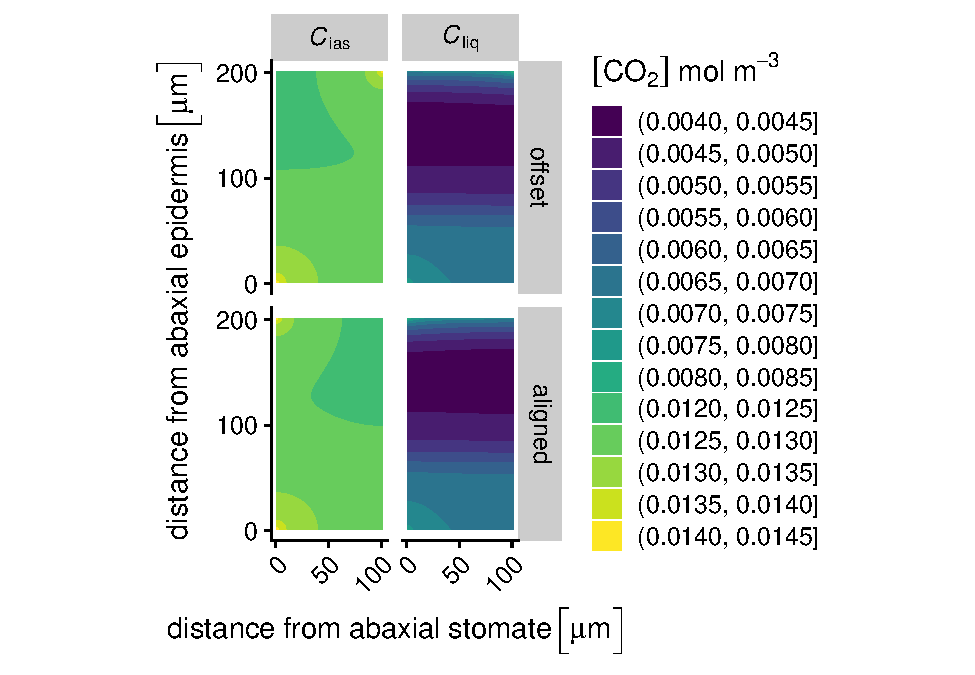
\includegraphics{figures/ph2d-example.pdf}

}

\caption{Example profiles of volumetric CO\(_2\) concentrations within
otherwise identical amphistomatous leaves that have stomatal positions
offset (top row) or aligned (bottom row) based on the 2-D porous medium
model. Stomatal positions are indicated by black points at the top and
bottom of panels. When stomata are aligned, both ab- and adaxial stomata
are position 0 along the \(x\)-axis; when stomata are offset, the
adaxial stomate is positioned \(U/2\) distance away. In this example,
variables are set as: \(I_0 = 1000\) \(\mu\)mol m\(^{-2}\) s\(^{-1}\);
\(\varphi_\text{pal} = 0.2\) m\(^3\) airspace m\(^{-3}\) leaf;
\(T_\text{leaf} = 200\) \(\mu\)m; \(U = 200\) \(\mu\)m. All other
parameter values are described in Table S1. \(C_\text{ias}\) =
{[}CO\(_2\){]} in intercellular airspace; \(C_\text{liq}\) =
{[}CO\(_2\){]} in chloroplast stroma; \(I_0\) = PPFD incident on the
leaf surface; \(\varphi_\text{pal}\) = Fraction of intercellular
airspace (aka porosity), palisade; \(T_\text{leaf}\) = Leaf thickness;
\(U\) = Interstomatal distance.}

\end{figure}

\begin{landscape}
\begin{longtable}[]{@{}
>{\raggedright\arraybackslash}p{(\columnwidth - 8\tabcolsep) * \real{0.29}}
>{\raggedright\arraybackslash}p{(\columnwidth - 8\tabcolsep) * \real{0.08}}
>{\raggedright\arraybackslash}p{(\columnwidth - 8\tabcolsep) * \real{0.1}}
>{\raggedright\arraybackslash}p{(\columnwidth - 8\tabcolsep) * \real{0.20}}
>{\raggedright\arraybackslash}p{(\columnwidth - 8\tabcolsep) * \real{0.33}}@{}}
\caption{Glossary of model terms and mathematical symbols.
}\tabularnewline
\toprule\noalign{}
\begin{minipage}[b]{\linewidth}\raggedright
Name
\end{minipage} & \begin{minipage}[b]{\linewidth}\raggedright
Symbol
\end{minipage} & \begin{minipage}[b]{\linewidth}\raggedright
Value
\end{minipage} & \begin{minipage}[b]{\linewidth}\raggedright
Units
\end{minipage} & \begin{minipage}[b]{\linewidth}\raggedright
Notes
\end{minipage} \\
\midrule\noalign{}
\endfirsthead
\toprule\noalign{}
\begin{minipage}[b]{\linewidth}\raggedright
Name
\end{minipage} & \begin{minipage}[b]{\linewidth}\raggedright
Symbol
\end{minipage} & \begin{minipage}[b]{\linewidth}\raggedright
Value
\end{minipage} & \begin{minipage}[b]{\linewidth}\raggedright
Units
\end{minipage} & \begin{minipage}[b]{\linewidth}\raggedright
Notes
\end{minipage} \\
\midrule\noalign{}
\endhead
\bottomrule\noalign{}
\endlastfoot
Whole-leaf light absorption & \(\alpha\) & \(0.8\) & mol mol\(^{-1}\) &
assumed \\
Chlorophyll spatial distribution coefficient & \(b_{0,\text{chl}}\) &
\(67.5\) & \(-\) & Borsuk and Brodersen (2019);
Equation~\ref{eq-Fchl} \\
Chlorophyll spatial distribution coefficient & \(b_{1,\text{chl}}\) &
\(41.5\) & \(-\) & Borsuk and Brodersen (2019);
Equation~\ref{eq-Fchl} \\
Chlorophyll spatial distribution coefficient & \(b_{2,\text{chl}}\) &
\(-29\) & \(-\) & Borsuk and Brodersen (2019); Equation~\ref{eq-Fchl} \\
Fraction of light absorbed by PSII & \(\beta\) & \(0.5\) & mol
mol\(^{-1}\) & assumed \\
{[}CO\(_2\){]} in intercellular airspace & \(C_\text{ias}\) & calculated
& mol m\(^{-3}\) & Equation~\ref{eq-2d_pm_flux} and
Equation~\ref{eq-fliq2} \\
{[}CO\(_2\){]} in chloroplast stroma & \(C_\text{liq}\) & calculated &
mol m\(^{-3}\) & Equation~\ref{eq-2d_pm_flux} \\
{[}CO\(_2\){]} in substomatal cavity & \(C_\text{stom}\) &
\(1.50 \times 10^{-2}\) & mol m\(^{-3}\) leaf & assumed \\
{[}CO\(_2\){]} compensation point & \(\Gamma^*\) &
\(1.35 \times 10^{-3}\) & mol m\(^{-3}\) stroma & Caemmerer (2000) \\
Diffusivity of {[}CO\(_2\){]} in intercellular airspace & \(D_\text{c}\)
& \(1.54 \times 10^{-5}\) & m\(^{2}\) s\(^{-1}\) & assumed \\
Effective diffusivity of {[}CO\(_2\){]} in intercellular airspace &
\(D_\text{e}\) & calculated & m\(^{2}\) s\(^{-1}\) &
Equation~\ref{eq-De} \\
Fraction of palisade mesophyll & \(f_\text{pal}\) & \(0.6\) & 1 &
\(1 = f_\text{pal} + f_\text{spg}\) \\
Fraction of spongy mesophyll & \(f_\text{spg}\) & \(0.4\) & 1 &
\(1 = f_\text{pal} + f_\text{spg}\) \\
Chlorophyll fluoresence profile along leaf depth normalized by total
fluoresence & \(F_\text{chl}\) & calculated & 1 & Borsuk and Brodersen
(2019); Equation~\ref{eq-Fchl} \\
Conductance of cell wall, plasmalemma, cytosol, chloroplast envelope,
and chloroplast stroma & \(g_\text{liq}\) & \(2.50 \times 10^{-4}\) &
m\(^3\) m\(^{-2}\) stroma s\(^{-1}\) & Evans et al. (2009) \\
PPFD incident on the leaf surface & \(I_0\) & variable & mol m\(^{-2}\)
s\(^{-1}\) & assumed \\
Potential photosynthetic e\(^{-}\) transport rate on a leaf area basis &
\(J_\infty\) & calculated & mol m\(^{-2}\) leaf s\(^{-1}\) &
Equation~\ref{eq-Jinf} \\
Maximum photosynthetic e\(^{-}\) transport rate on a leaf area basis &
\(J_\text{max}\) & \(2.75 \times 10^{-4}\) & mol m\(^{-2}\) leaf
s\(^{-1}\) & assumed \\
Effective photosynthetic e\(^{-}\) transport rate on a stroma volume
basis & \(j_\text{e}\) & calculated & mol m\(^{-3}\) stroma s\(^{-1}\) &
Equation~\ref{eq-je} \\
Potential photosynthetic e\(^{-}\) transport rate on a stroma volume
basis & \(j_\infty\) & calculated & mol m\(^{-3}\) stroma s\(^{-1}\) &
Equation~\ref{eq-Jinf} \\
Maximum photosynthetic e\(^{-}\) transport rate on a stroma volume basis
& \(j_\text{max}\) & calculated & mol m\(^{-3}\) stroma s\(^{-1}\) &
Equation~\ref{eq-jmax} \\
Catalytic rate of Rubisco & \(k_\text{c}\) & \(2.84\) & m\(^{-1}\) &
Tholen and Zhu (2011) \\
Rubisco effective \(K_\text{m}\) & \(K_\text{m}\) &
\(1.87 \times 10^{-2}\) & mol m\(^{-3}\) & Caemmerer (2000) \\
Number of elements in \(x\) direction & \(n_x\) & calculated & \(-\) &
\(U = 2 n_x t_\text{elem}\) \\
Number of elements in \(z\) direction & \(n_z\) & calculated & \(-\) &
\(T_\text{leaf} = n_z t_\text{elem}\) \\
Fraction of intercellular airspace (aka porosity), palisade &
\(\varphi_\text{pal}\) & variable & m\(^3\) airspace m\(^{-3}\) leaf &
assumed \\
Fraction of intercellular airspace (aka porosity), spongy &
\(\varphi_\text{spg}\) & \(0.3\) & m\(^3\) airspace m\(^{-3}\) leaf &
assumed \\
Quantum yield of PSII e\(^{-}\) transport & \(\phi_\text{PSII}\) &
\(0.85\) & mol mol\(^{-1}\) & assumed \\
Volumetric rate of RuBP carboxylation & \(r_\text{c}\) & calculated &
mol m\(^{-2}\) stroma s\(^{-1}\) & Equation~\ref{eq-rc} \\
Volumetric respiration rate & \(r_\text{d}\) & \(6.60 \times 10^{-2}\) &
mol m\(^{-2}\) stroma s\(^{-1}\) & Earles et al. (2017); Tholen and Zhu
(2011) \\
Volumetric rate of photorespiratory CO\(_2\) release & \(r_\text{p}\) &
calculated & mol m\(^{-2}\) stroma s\(^{-1}\) & Earles et al. (2017);
Equation~\ref{eq-rp} \\
Mesophyll surface area-to-leaf surface area ratio, palisiade &
\(S_\text{m,pal}\) & \(20\) & m\(^2\) mesophyll m\(^{-2}\) leaf &
assumed \\
Mesophyll surface area-to-leaf surface area ratio, spongy &
\(S_\text{m,spg}\) & \(2\) & m\(^2\) mesophyll m\(^{-2}\) leaf &
assumed \\
Tortuosity of intercellular airspace & \(\tau\) & \(1.55\) & m
m\(^{-1}\) & Syvertsen et al. (1995) \\
Thickness of element in both \(x\) and \(z\) directions &
\(t_\text{elem}\) & \(1.00 \times 10^{-6}\) & m &
\(T_\text{leaf} = n_z t_\text{elem}\) \\
Leaf thickness & \(T_\text{leaf}\) & variable & m &
\(T_\text{leaf} = n_z t_\text{elem}\) \\
Interstomatal distance & \(U\) & variable & m &
\(U = n_x t_\text{elem}\) \\
Stroma volume-to-mesophyll surface area ratio & \(V_\text{strom}\) &
\(1.74 \times 10^{-6}\) & m\(^3\) stroma m\(^{-2}\) mesophyll & Earles
et al. (2017); Tholen and Zhu (2011) \\
Rubisco-limited carboxylation rate & \(w_\text{c}\) & calculated & mol
m\(^{-2}\) stroma s\(^{-1}\) & Equation~\ref{eq-wc} \\
RuBP regeneration-limited carboxylation rate & \(w_\text{j}\) &
calculated & mol m\(^{-2}\) stroma s\(^{-1}\) & Equation~\ref{eq-wj} \\
Rubisco concentration in stroma & \(X_\text{c}\) & \(2.5\) & mol
m\(^{-3}\) stroma & Tholen and Zhu (2011); Oguchi, Hikosaka, and Hirose
(2003) \\
\end{longtable}
\end{landscape}

\newpage

\hypertarget{references}{%
\subsection*{References}\label{references}}
\addcontentsline{toc}{subsection}{References}

\hypertarget{refs}{}
\begin{CSLReferences}{1}{0}
\leavevmode\vadjust pre{\hypertarget{ref-borsuk_spatial_2019}{}}%
Borsuk, Aleca M., and Craig R. Brodersen. 2019. {``The Spatial
Distribution of Chlorophyll in Leaves.''} \emph{Plant Physiology} 180
(3): 1406--17. \url{https://doi.org/10.1104/pp.19.00094}.

\leavevmode\vadjust pre{\hypertarget{ref-von_caemmerer_biochemical_2000}{}}%
Caemmerer, Susanne von. 2000. \emph{Biochemical Models of Leaf
Photosynthesis}. Techniques in Plant Science 2. Collingwood: CSIRO.

\leavevmode\vadjust pre{\hypertarget{ref-earles_excess_2017}{}}%
Earles, J. Mason, Guillaume Théroux-Rancourt, Matthew E. Gilbert, Andrew
J. McElrone, and Craig R. Brodersen. 2017. {``Excess Diffuse Light
Absorption in Upper Mesophyll Limits {CO}\(_{\textrm{2}}\) Drawdown and
Depresses Photosynthesis.''} \emph{Plant Physiology} 174 (2): 1082--96.
\url{https://doi.org/10.1104/pp.17.00223}.

\leavevmode\vadjust pre{\hypertarget{ref-evans_resistances_2009}{}}%
Evans, J. R., R. Kaldenhoff, B. Genty, and I. Terashima. 2009.
{``Resistances Along the {CO}\(_{\textrm{2}}\) Diffusion Pathway Inside
Leaves.''} \emph{Journal of Experimental Botany} 60 (8): 2235--48.
\url{https://doi.org/10.1093/jxb/erp117}.

\leavevmode\vadjust pre{\hypertarget{ref-johnson_leaf_2005}{}}%
Johnson, Daniel M., William K. Smith, Thomas C. Vogelmann, and Craig R.
Brodersen. 2005. {``Leaf Architecture and Direction of Incident Light
Influence Mesophyll Fluorescence Profiles.''} \emph{American Journal of
Botany} 92 (9): 1425--31. \url{https://doi.org/10.3732/ajb.92.9.1425}.

\leavevmode\vadjust pre{\hypertarget{ref-nishio_carbon_1993}{}}%
Nishio, J. N., J. Sun, and T. C. Vogelmann. 1993. {``Carbon {Fixation}
{Gradients} Across {Spinach} {Leaves} {Do} {Not} {Follow} {Internal}
{Light} {Gradients}.''} \emph{The Plant Cell}, August, 953--61.
\url{https://doi.org/10.1105/tpc.5.8.953}.

\leavevmode\vadjust pre{\hypertarget{ref-oguchi_does_2003}{}}%
Oguchi, R., K. Hikosaka, and T. Hirose. 2003. {``Does the Photosynthetic
Light-Acclimation Need Change in Leaf Anatomy?: {Chloroplast} Volume
Change in Photosynthetic Light-Acclimation.''} \emph{Plant, Cell \&
Environment} 26 (4): 505--12.
\url{https://doi.org/10.1046/j.1365-3040.2003.00981.x}.

\leavevmode\vadjust pre{\hypertarget{ref-soetaert_practical_2009}{}}%
Soetaert, Karline, and Peter M. J. Herman, eds. 2009. \emph{A
{Practical} {Guide} to {Ecological} {Modelling}}. Dordrecht: Springer
Netherlands. \url{https://doi.org/10.1007/978-1-4020-8624-3}.

\leavevmode\vadjust pre{\hypertarget{ref-syvertsen_relationship_1995}{}}%
Syvertsen, J. P., J. Lloyd, C. McConchie, P. E. Kriedemann, and G. D.
Farquhar. 1995. {``On the Relationship Between Leaf Anatomy and
{CO}\(_{\textrm{2}}\) Diffusion Through the Mesophyll of Hypostomatous
Leaves.''} \emph{Plant, Cell and Environment} 18 (2): 149--57.
\url{https://doi.org/10.1111/j.1365-3040.1995.tb00348.x}.

\leavevmode\vadjust pre{\hypertarget{ref-tholen_mechanistic_2011}{}}%
Tholen, D., and X.-G. Zhu. 2011. {``The Mechanistic Basis of Internal
Conductance: {A} Theoretical Analysis of Mesophyll Cell Photosynthesis
and {CO}\(_{\textrm{2}}\) Diffusion.''} \emph{Plant Physiology} 156 (1):
90--105. \url{https://doi.org/10.1104/pp.111.172346}.

\leavevmode\vadjust pre{\hypertarget{ref-wood_generalized_2017}{}}%
Wood, Simon N. 2017. \emph{Generalized {Additive} {Models}: {An}
{Introduction} with {R}}. 2nd ed. Chapman; Hall/CRC.
\url{https://doi.org/10.1201/9781315370279}.

\end{CSLReferences}



\end{document}
